%%%%%%%%%%%%%%%%%%%%%%%%%
% Dokumentinformationen %
%%%%%%%%%%%%%%%%%%%%%%%%%
\newcommand{\titleinfo}{Vorlage}
\newcommand{\authorname}{\href{mailto:lmazzole@hsr.ch}{L. Mazzoleni}}
\newcommand{\authoremail}{\href{mailto:lmazzole@hsr.ch}{lmazzole@hsr.ch} }
\newcommand{\versioninfo}{$ Revision: 1.1 $}

%\newcommand{\authorinfo}{Stefan Reinli \texttt{stefan.reinlil@hsr.ch}\\Luca Mazzoleni \texttt{luca.mazzoleni@hsr.ch}}
%NEWCOMMANDS überarbeiten
%wieso mit new Command? Author Email Info besser aufteilen

%%%%%%%%%%%%%%%%%%%%%%%%%%%%%%%%%%%%%%%%%%%%%
% Standard projektübergreifender Header für 
% - Makros 
% - Farben
% - Mathematische Operatoren
%
% dORT NUR ERGÄNZEN, NICHTS LÖSCHEN
%%%%%%%%%%%%%%%%%%%%%%%%%%%%%%%%%%%%%%%%%%%%%
%BuG-Fix
%Package pdf Error: Driver file ................ not found
%If you have a luatex driver fail uncomment these lines
\RequirePackage{luatex85}
\def\pgfsysdriver{pgfsys-pdftex.def}

% Genereller Header
\documentclass[11pt,twoside,a4paper,fleqn]{article}
% Dateiencoding
\usepackage[utf8]{inputenc}
\usepackage[T1]{fontenc}	%ä,ü...
% Seitenränder
\usepackage[left=1cm,right=1cm,top=0.5cm,bottom=0.5cm,includeheadfoot]{geometry}
% Sprachpaket 
\usepackage[english, ngerman]{babel} % Silbentrennung und Rechtschreibung Englisch und Deutsch

%%%%%%%%%%%%%%%%%%%%%%%
%% Wichtige Packages %%
%%%%%%%%%%%%%%%%%%%%%%%
\usepackage{amsmath}                % Allgemeine Matheumgebungen									
\usepackage{amssymb}                % Fonts: msam,msbm, eufm & Mathesymbole, Mengen (lädt automatisch amsfonts)									
\usepackage{array}                  % \newcolumntype, \firsthline, ,\lasthline, m{width}, b{width}									
\usepackage{caption}                % Bildunterschriften									
\usepackage{enumitem}               % basic environments: enumerate, itemize, description									
\usepackage{fancybox}               % \fbox: \shad­ow­box, \dou­ble­box, \oval­box, \Oval­box									
\usepackage{fancyhdr}               % Seiten schöner gestalten, insbesondere Kopf- und Fußzeile									
\usepackage{floatflt}               % Textumflossene Abbildungen \begin{floatingfigure}[r]{Breite} : r rechts, l links, p links auf geraden Seiten und rechts auf ungeraden Seiten								
\usepackage{graphicx}               % \includegraphics[keyvals]{imagefile}, [draft]graphicx zeigt nur Namen und Rahmen an, [final] hebt diese option auf => Bild wird angezeigt    									
\usepackage{hyperref}               % Erstellt Verweise innerhalb und nach außerhalb eines PDF Dokumentes.									
\usepackage{lastpage}               % Bspw. : Page 1 of 3 => \thepage\ of \pageref{LastPage}									
\usepackage{listings}               % Erlaubt es Programmcode in der gewünschten Sprache zu hinterlegen (C++, Matlab,..). Definition der Sprache mit \lstset{language=name}..									
\usepackage{longtable}              % Longtable erlaubt es Tabellen zu erstellen die bei der nächsten Seite weiterlaufen. (Bricht automatisch um)									
\usepackage{mathabx}                % Mathesymbole									
\usepackage{mathrsfs}               % \mathscr (Benötigt für Fourierreihen-Symbol)									
%\usepackage{mathtools}              % Extension package to amsmath									
\usepackage{multicol}               % multicols-Umgebung \begin{multicols}{3} erzeugt Abschnitt mit 3 Spalten									
\usepackage{multirow}               % Tabelle: ermöglicht es Felder mehrerer Zeilen in einem zusammenzufassen									
\usepackage{pdflscape}              % adds PDF support to the environment 'landscape'									
\usepackage{pxfonts}                % Symbole, griechisches Alphabet, Integrale...									
\usepackage{rotating}               % sideways, turn{degree}, rotate{degree}, sidewaysfigure, sidewaystable Umgebung									
\usepackage{subcaption}             % Bildunterschriften für Subfigures									
\usepackage{tabularx}               % tabularx-Umgebung: Hat feste Gesamtbreite, \begin{tabularx}{\textwidth}{c c c c c} X: Spalte mit variabler Breite, l, c, r, p{breite}, m{breite}									
\usepackage{textcomp}               % text symbols: baht, bullet, copyright, musical-note, onequarter, section, yen									
\usepackage{tikz}                   % Tikz Umgebung zur Grafikerzeugung									
\usepackage{titlesec}               % Überschriften zu Textabstände
\usepackage{trfsigns}               % Transformationszeichen \laplace, \Laplace..									
\usepackage{trsym}                  % Weitere Laplace Zeichen erlaubt auch vertikale Transformationszeichen									
\usepackage{verbatim}               % verbatim, verbatim*, comment Umgebung									
\usepackage{wrapfig}                % Textumflossene Bilder und Tabellen, \begin{wrapfigure}[Zeilen]{Position}[Ueberhang]{Breite}									
\usepackage{xcolor}                 % \pagecolor{color}, \textcolor{color}{text}, \colorbox{color}{text}, \fcolorbox{border-color}{fill-color}{text}									
\usepackage{titlesec}
% Zum Bilder einfach in Tabellen einfügen (valign=t)
\usepackage[export]{adjustbox}

%%%%%%%%%%%%%%%%%%%%
% Generelle Makros %
%%%%%%%%%%%%%%%%%%%%
\newcommand{\skript}[1]{$_{\textcolor{red}{\mbox{\small{Skript S.#1}}}}$}
\newcommand{\verweis}[2]{\small{(siehe auch \ref{#1}, #2 (S. \pageref{#1}))}}
\newcommand{\verweiskurz}[1]{(\small{siehe \ref{#1}\normalsize)}}
\newcommand{\subsubadd}[1]{\textcolor{black}{\mbox{#1}}}
\newcommand{\formelbuch}[1]{$_{\textcolor{red}{\mbox{\small{S#1}}}}$}

\newcommand{\kuchling}[1]{$_{\textcolor{red}{\mbox{\small{Kuchling #1}}}}$}
\newcommand{\stoecker}[1]{$_{\textcolor{grey}{\mbox{\small{Stöcker #1}}}}$}
\newcommand{\sachs}[1]{$_{\textcolor{blue}{\mbox{\small{Sachs S. #1}}}}$}
\newcommand{\hartl}[1]{$_{\textcolor{green}{\mbox{\small{Hartl S. #1}}}}$}

\newcommand{\schaum}[1]{\tiny Schaum S. #1}

\newcommand{\skriptsection}[2]{\section{#1 {\tiny Skript S. #2}}}
\newcommand{\skriptsubsection}[2]{\subsection{#1 {\tiny Skript S. #2}}}
\newcommand{\skriptsubsubsection}[2]{\subsubsection{#1 {\tiny Skript S. #2}}}

\newcommand{\matlab}[1]{\footnotesize{(Matlab: \texttt{#1})}\normalsize{}}

% Syntax: \bmu{Pfad zum Bild}{Bildgrösse}{Beschriftung des Bildes}
\newcommand{\bl}[2]{
	\begin{figure}[h]
		\flushleft  % linksbuendig
		\includegraphics[width=#1]{#2} \\
	\end{figure}
}
\newcommand{\br}[2]{
	\begin{figure}[h]
		\flushright  % rechtsbuendig
		\includegraphics[width=#1]{#2} \\
	\end{figure}
}

\newcommand{\bild}[2]{
	\begin{figure}[h]
		\centering  % zentriert
		\includegraphics[width=#1]{#2} \\
	\end{figure}
}

\newcommand\tabbild[2][]{%
	\raisebox{0pt}[\dimexpr\totalheight+\dp\strutbox\relax][\dp\strutbox]{%
		\includegraphics[#1]{#2}%
	}%
}

\newcolumntype{P}[1]{>{\raggedright\arraybackslash}p{#1}} %Tabelle linksausgerichtet
\newcolumntype{L}[1]{>{\raggedleft\arraybackslash}p{#1}} %Tabelle rechtsausgerichtet
\newcolumntype{C}[1]{>{\centering\arraybackslash}p{#1}}



%%%%%%%%%%
% Farben %
%%%%%%%%%%
\definecolor{black}{rgb}{0,0,0}
\definecolor{red}{rgb}{1,0,0}
\definecolor{white}{rgb}{1,1,1}
\definecolor{grey}{rgb}{0.8,0.8,0.8}
\definecolor{green}{rgb}{0,.8,0.05}
\definecolor{brown}{rgb}{0.603,0,0}
\definecolor{mymauve}{rgb}{0.58,0,0.82}


%%%%%%%%%%%%%%%%%%%%%%%%%%%%
% Mathematische Operatoren %
%%%%%%%%%%%%%%%%%%%%%%%%%%%%
\DeclareMathOperator{\sinc}{sinc}
\DeclareMathOperator{\sgn}{sgn}
\DeclareMathOperator{\Real}{Re}
\DeclareMathOperator{\Imag}{Im}
%\DeclareMathOperator{\e}{e}
\DeclareMathOperator{\cov}{cov}
\DeclareMathOperator{\PolyGrad}{PolyGrad}

%Grösse Integral anpassen
\def\Int{\mbox{\Large$\displaystyle\int$\normalsize}}
\def\OInt{\mbox{\Large$\displaystyle\oint$\normalsize}}

%Makro für 'd' von Integral- und Differentialgleichungen 
\newcommand*{\diff}{\mathop{}\!\mathrm{d}}

%%%%%%%%%%%%%%%%%%%%%%%%%%%
% Fouriertransformationen %
%%%%%%%%%%%%%%%%%%%%%%%%%%%

% Fouriertransformationen
\unitlength1cm
\newcommand{\FT}
{
	\begin{picture}(1,0.5)
	\put(0.2,0.1){\circle{0.14}}\put(0.27,0.1){\line(1,0){0.5}}\put(0.77,0.1){\circle*{0.14}}
	\end{picture}
}


\newcommand{\IFT}
{
	\begin{picture}(1,0.5)
	\put(0.2,0.1){\circle*{0.14}}\put(0.27,0.1){\line(1,0){0.45}}\put(0.77,0.1){\circle{0.14}}
	\end{picture}
}


%%%%%%%%%%%%%%%%%%%%%%%%%%%%
% Allgemeine Einstellungen %
%%%%%%%%%%%%%%%%%%%%%%%%%%%%

%Pdf Info
\hypersetup{pdfauthor={\authorname},pdftitle={\titleinfo},colorlinks=false}
\author{\authorname}
\title{\titleinfo}

% Abstände Text zu Übertiteln / Einzug
\titlespacing{\section}{12pt}{1em}{0.5em}
\titlespacing{\subsection}{12pt}{1em}{0.5em}
\titlespacing{\subsubsection}{12pt}{1em}{0.5em}

%%%%%%%%%%%%%%%%%%%%%%%
% Kopf- und Fusszeile %
%%%%%%%%%%%%%%%%%%%%%%%
\pagestyle{fancy}
\fancyhf{}
%Linien oben und unten
\renewcommand{\headrulewidth}{0.5pt} 
\renewcommand{\footrulewidth}{0.5pt}

%Kopfzeile links bzw innen
\fancyhead[L]{\titleinfo{ }\tiny{(\versioninfo)}}
%Kopfzeile mitte
%\fancyhead[C]{}
%Kopfzeile rechts bzw. aussen
\fancyhead[R]{Seite \thepage { }von \pageref{LastPage}}

%Fusszeile links bzw. innen
\fancyfoot[L]{\footnotesize{\authorname}}
%Fusszeile mitte
%\fancyfoot[C]{\footnotesize{\authoremail}}
%Fusszeile rechts bzw. ausen
\fancyfoot[R]{\footnotesize{\today}}
% Einrücken verhindern versuchen
\setlength{\parindent}{0pt}

%%%%%%%%%%%%%%%%%%%%%%%%%%%%%%%%%%%%%%%
%% Makros & anderer Low-Level bastel %%
%%%%%%%%%%%%%%%%%%%%%%%%%%%%%%%%%%%%%%%
% Zeilenhöhe Tabellen:
\newcommand{\arraystretchOriginal}{1.5}
\renewcommand{\arraystretch}{\arraystretchOriginal}

\makeatletter
%% Makros für den Arraystretch (bei uns meist in Tabellen genutzt, welche Formeln enthalten)
% Default Value
\def\@ArrayStretchDefault{1} % Entspricht der Voreinstellung von Latex

% Setzt einen neuen Wert für den arraystretch
\newcommand{\setArrayStretch}[1]{\renewcommand{\arraystretch}{#1}}

% Setzt den arraystretch zurück auf den default wert
\newcommand{\resetArrayStretch}{\renewcommand{\arraystretch}{\@ArrayStretchDefault}}

% Makro zum setzten des Default arraystretch. Kann nur in der Präambel verwendet werden.
\newcommand{\setDefaultArrayStretch}[1]{%
    \AtBeginDocument{%
        \def\@ArrayStretchDefault{#1}
        \renewcommand{\arraystretch}{#1}
    }
}
\makeatother

% Settings which are used to set the distance above and under the sections
%\titlespacing*{\paragraph}{0pt}{2.25ex plus 1ex minus .2ex}{1.0ex plus .2ex}
\titlespacing{\section}{0em}{0.5em}{0.5em}
\titlespacing{\subsection}{0em}{0.5em}{0.5em}
\titlespacing{\subsubsection}{0em}{0.5em}{0.5em}
% Linksb�ndig
\setlength\parindent{0ex}

%To delete the whitespace before an Itemize
\setlist[itemize]{noitemsep, topsep=0pt}
%% Achtung Symbol \danger
\newcommand*{\TakeFourierOrnament}[1]{{%
        \fontencoding{U}\fontfamily{futs}\selectfont\char#1}}
\newcommand*{\danger}{\TakeFourierOrnament{66}}
%\usepackage{circuitikz}
% Möglichst keine Ergänzungen hier, sondern in header.tex

%%%%%%%%%%%%%%%%%%%%%%%%%%%%%%%%%%%%%%%%%%%%%%%%%%%%%%%%%%%%%%%%%%%%%%%%%%%%%%%%%%%%%%%%%%%%%%%%
%%%%%%%%%%%%%%%%%%%%%%%%%%%%%%%%%%%%%%%%%%%%%%%%%%%%%%%%%%%%%%%%%%%%%%%%%%%%%%%%%%%%%%%%%%%%%%%%

\begin{document}
\maketitle
\tableofcontents
\thispagestyle{empty}
\newpage
\section{V1}
\subsection{Anwendung und Grundlage der uP-Technik}

\begin{minipage}{8cm}
    \subsection{Aufbau}
    Verstehe die wesentlichen Systemkomponetnen des Rechnersystems auf einem IC (Integrated Circuit)
\end{minipage}
\begin{minipage}{0.5\linewidth}
    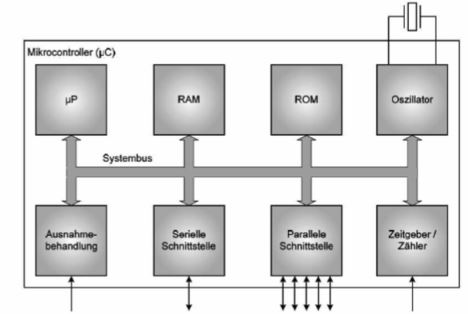
\includegraphics[width=\linewidth]{images/aufbauuC}
\end{minipage}

\begin{multicols}{2}
\subsubsection{Anwendungen}
\begin{minipage}{\linewidth}
\begin{itemize}
    \item Supercomputer
    \item Arbeits und Server-Rechnern
    \item Smartphones
    \item Navigationssysteme
    \item Digitalkameras
    \item Drucker
    \item ...
\end{itemize}
\end{minipage}

\begin{minipage}{\linewidth}
\subsubsection{Aufbau von uP-basierten Systemen}
\begin{itemize}
    \item Zentraleinheit CPU mit
    \begin{itemize}
        \item Rechenwerk ALU
        \item Steuerwerk CU
        \item Registersatz
    \end{itemize}
    \item Speicher
    \item Eingabe-/Ausgabe-Schnittsellen
\end{itemize}
\end{minipage}
\end{multicols}

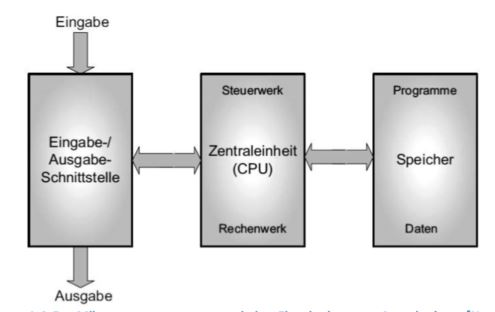
\includegraphics[width=0.5\linewidth]{images/aufbauuC1}
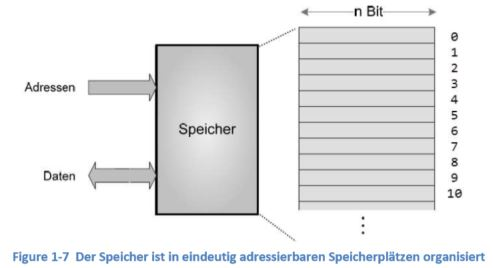
\includegraphics[width=0.5\linewidth]{images/aufbauuCspeicher}

\subsubsection{Havard vs Von Neumann Architektur}
\begin{multicols}{2}
    \begin{minipage}{\linewidth}
        \textbf{Harvard Rechnermodell}\\
        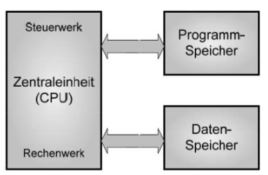
\includegraphics[width=0.6\linewidth]{images/HavardArchi}
    \end{minipage}
    
    \begin{minipage}{\linewidth}
        \textbf{von Neumann Rechnermodell}\\
        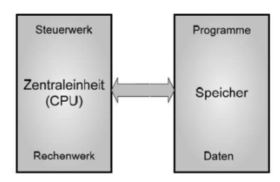
\includegraphics[width=0.6\linewidth]{images/NeumannArchi}
    \end{minipage}
\end{multicols}
\clearpage
%===================================
\subsubsection{Programmierung eins uP}
\begin{multicols}{2}
\begin{minipage}{\linewidth}
    Ein $\mu$ P kann durch individuelle Programmierung auf ganz unterschiedliche Art angepasst werden. \newline
    $\rightarrow$ entscheidend für die Durchdringung im Markt.\newline
    Ein Programm enthält in aufeinanderfolgender Anordnung die Maschinen-Befehle oder -Instruktionen für den $\mu$ P. Diese Maschiene-Befehle teilen der CPU mit, welche Operationen in welcher Reihenfolge und auf welche Daten angewendet werden sollen. \newline
    Die Befehlsfolge des Programms wird innerhalb der CPU vom Steuerwerk gesteuert und schrittweise ausgeführt. Dazu wird der aktuell zur bearbeitende Befehl durch einen Programmzähler (PC) im Speicher adressiert.\newline
    Der PC enthält laufend die Adresse der Speicherzelle des jeweiligen Befehls im Speicher.
\end{minipage}

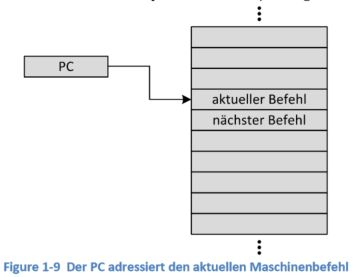
\includegraphics[width=\linewidth]{images/uPPC}
\end{multicols}
    
\subsubsection{Befehlsformate}
\begin{multicols}{2}
\begin{minipage}{\linewidth}
Die Art und Wirkung eines Befehls wird im Befehlswort (\textbf{OpCode}) codiert.
Darin sind neben der Operation auch die Operanden spezifiziert.
Die Codierung des Befehlswortes erfolgt abhängig vom $\mu$ P.
Der Maschinencode setzt sich aus einem OpCode und einem oder mehreren Operanden zusammen.
\end{minipage}

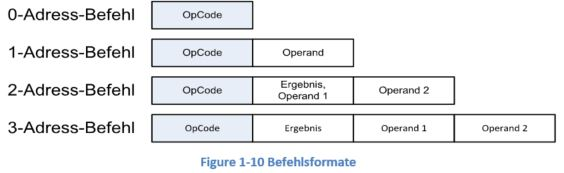
\includegraphics[width=\linewidth]{images/Befehlsformate}
\end{multicols}


\subsection{RISC vs CISC}
\begin{multicols}{2}
    \textbf{CISC}\newline
    Complex Instruction Set Computer
    \\
    \textbf{RISC}\newline
    Reduced Instruction Set Computer
\end{multicols}
\subsubsection{RISC-Rechner}
effizienter als CISC-Rechner
\begin{itemize}
    \item besteht aus einer kleinen Anz. von Befehlen mit wenigen Adressierungsarten
    \item Registersatz enthält eine grosse Anzahl von allg. verwendbaren Registern\newline
    General Purpose Register (GPR)
    \item Speicherzugriff erfolgt über spezielle Lade- und Speicher-Befehle
    \begin{itemize}
        \item Arithmetisch-logische Operationen arbeiten auf Registeroperanden
    \end{itemize}
    \item Pipeline-Architecture $\leftarrow$ Leistungssteigernde Architektur
    \item Eine grosse semantische Lücke entsteht bei der Übersetzung aus der Hochsprache
\end{itemize}

\subsubsection{u Architektur}
Beschreibt die architektonischen Details bei der Implementierung der $\mu$ P aus Sicht der Programmierer.
Dies umfasst die Beschreibung der Zentraleinheit (CPU), des Rechenwerks (ALU) und des Steuerwerks (CU).


\clearpage

\subsection{Hardware}
\begin{minipage}[t]{10cm}
	\subsubsection{Registersatz}
	Register sind schnelle Zwischenspeicher für \newline
	temporäre Daten im $\mu$ P.
\end{minipage}
\begin{minipage}[t]{0.5\linewidth}
	\subsubsection{Hardware- /Software-Schnitsttelle}
	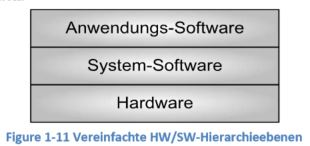
\includegraphics{images/HardwareSoftware}
\end{minipage}

\subsubsection{Taktfrequenz}
Das Taktsignal steuert die zeitliche Abfolge im $\mu$ P \newline
\begin{multicols}{2}
        \begin{minipage}{\linewidth}
    \[ f_{Takt}= \frac{1}{T_{takt}} \]
        \end{minipage}
    
    \begin{minipage}{\linewidth}
        $ \Uparrow $ Taktrate \-\ $ \Leftrightarrow $ \-\ $  \Uparrow  $Leistungsaufnahme \\
        Um Energie zu sparen ist es sinnvoll die Taktrate laufend anzupassen.\\
    \end{minipage}
\end{multicols}
\subsubsection{Leistungsaufnahme}
\begin{multicols}{2}
        \begin{minipage}{\linewidth}
\[ P_{Gate}= \frac{1}{2} \cdot C_{Last} \cdot V_{DD}^2\cdot f_{Takt} \]
    \end{minipage}
    
\begin{minipage}{\linewidth}
    $ P_{Gate} \qquad $Leistung pro CMOS Gate \newline
    $ C_{Last} \qquad $Lastkapazität\newline
    $ V_{DD}   \qquad $Versorgungsspannung\newline
    $ f_{Takt} \qquad $Taktfrequenz
\end{minipage}
\end{multicols}

\subsection{Software}
\begin{minipage}[b]{11cm}
	\subsubsection{Ablauf}
	\begin{itemize}
    	\item Der \textbf{Präprozessor} bereitet das Quellprogramm für den Compiler vor
    	\item Der \textbf{Compiler} übersetzt das Programm von einer Hochsprache in ein Assembly-Programm
    	\item Der \textbf{Binder} fasst verschiedene Dateien, die verschiebbaren Maschinencode enthalten, zu einem Programm zusammen.
    	\item Der \textbf{Loader} wandelt die verschiebbaren Adressen in absolute Adressen um und lädt sie in den Speicher des Systems.
	\end{itemize}
\end{minipage}
%
\begin{minipage}{0.5cm}
	\-\
\end{minipage}
%
\begin{minipage}{7cm}
	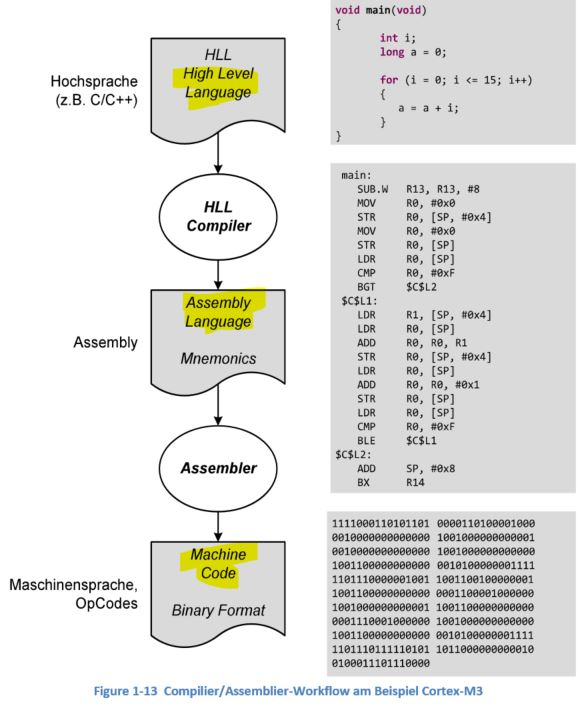
\includegraphics[width=\linewidth]{images/CompilerWorkflow}
\end{minipage}






















    
\section{V3}
\subsection{Halbleiter Speicher}
\begin{multicols}{2}
\textbf{Zentraler Speicher}
\begin{itemize}
    \item direkt am Bussystem angeschlossen
\end{itemize}
\textbf{Peripherer Speicher}
\begin{itemize}
    \item über I/O-Schnittstelle angeschlossen
\end{itemize}

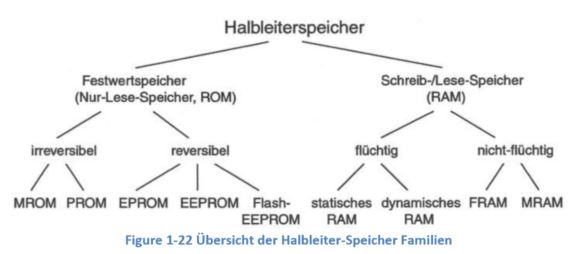
\includegraphics[width=10cm]{images/halbleiterfam}
\end{multicols}

\begin{multicols}{2}
\subsubsection{ROM-Festwertspeicher}
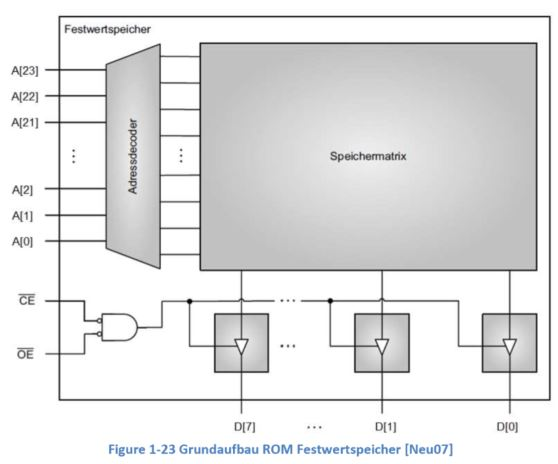
\includegraphics[width=8cm]{images/ROM}

\subsubsection{RAM-Speicher-/Lese-Speicher}
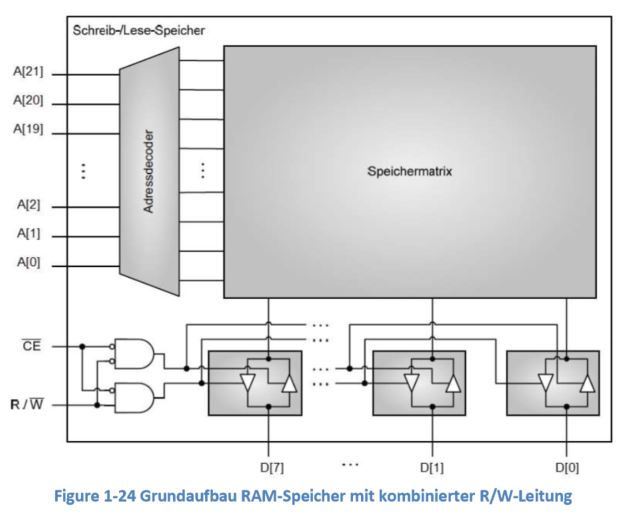
\includegraphics[width=8cm]{images/RAM}
\end{multicols}

\subsection{Speicherorganisation}
\begin{multicols}{2}
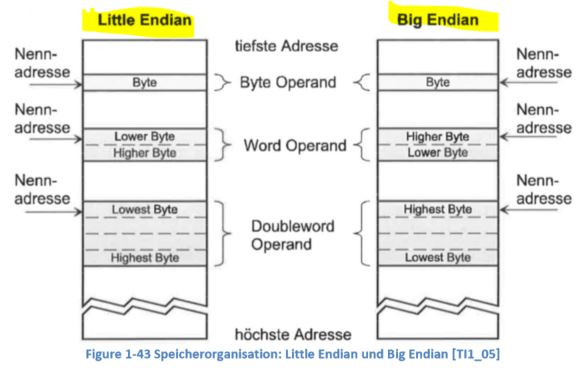
\includegraphics[width=8cm]{images/LittleBigEndian}

\subsubsection{I/O - Schnittstelle}
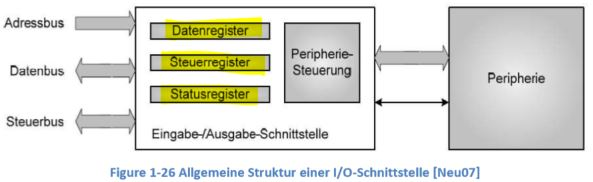
\includegraphics[width=8cm]{images/IOSchnittstelle}
\end{multicols}

\includegraphics{images/Speicherraumadressierung}
\section{Cortex}
\subsection{Cortex M Varianten}
\begin{multicols}{2}
\textbf{Cortex M0 und M0+}
    \begin{itemize}
        \item kleinster Vertreter der CortexFam
        \item Ersatz von 8Bit- uC
        \end{itemize}                     
 \textbf{Cortex M1}
    \begin{itemize}
        \item als Softcore Implementiert
        \item Vergleichbar mit Cortex-M0
    \end{itemize}
\end{multicols}
\begin{multicols}{2}
   \textbf{Cortex M3}     
     \begin{itemize}
         \item erster Vertreter der CortexFam
         \item 32 Bit Architektur
         \item ersetzt 8 \& 16 Bit uC
         \item Thumb ISA (Instruction Set Architecure)\newline
         Mix aus 16 und 32BIt langen anweisungen
     \end{itemize}   
               
   \textbf{Cortex M4} 
    \begin{itemize}
        \item vergleichbar mit M3 jedoch mit
        \qquad\item Digital Signal Processing (DSP)
        \qquad\item Floating Point Unit (FPU)
        \newline
      \end{itemize}  
\end{multicols}
\clearpage
\begin{multicols}{2}
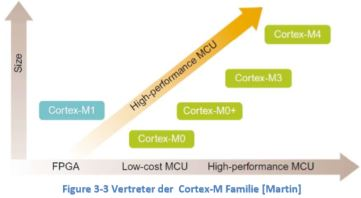
\includegraphics[width=\linewidth]{images/cortexmfam}

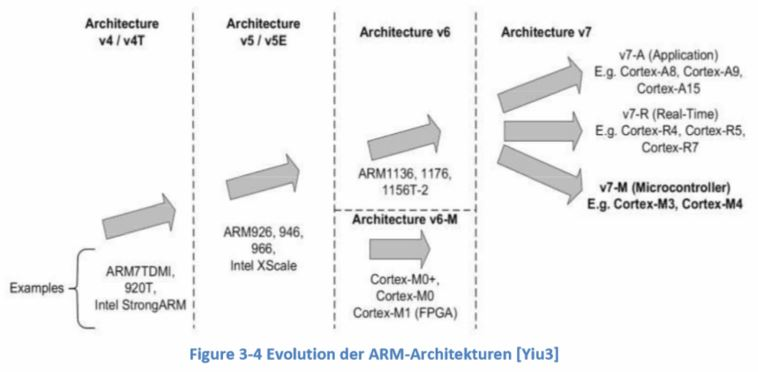
\includegraphics[width=\linewidth]{images/cortexmcomp}
\end{multicols}

\begin{multicols}{3}
    \textbf{Cortex-A}
    \begin{itemize}
        \item HighEnd Anwendungen und Betriebssysteme
        \item hohe Rechenleistung
        \item Chache Memory
    \end{itemize}
    
    \textbf{Cortex-R}
    \begin{itemize}
       \item Echtzeitfähigkeit
       \item hohe Zuverlässigkeit
       \item System on Chip (SOC) 
    \end{itemize}  
    
        \textbf{Cortex-M}
        \begin{itemize}
            \item Speziell für \mu C-Markt
            \item Low Cost, Low Energy
            \item System on Chip (SOC) 
          \end{itemize}             
\end{multicols}
\subsubsection{Vorteile der Cortex-M-Prozessoren}
\begin{itemize}
    \item Low Power
        \subitem < 200\mu A / MHz
    \item Performance
        \subitem >1.25 DMIPS / MHz
    \item Energy Efficiency
        \subitem low Power, high performance
    \item Code Density
        \subitem Thumb 2 Befehlssatz
    \item Interrupts
        \subitem 240 Interrupts
    \item Easy of Use, C Friedly
    \item Scalability
    \item Debug Features
    \item Software portability and Reusebility
    \item OS Support
    \item Choices (Derivers, Tools, OS,..)    
\end{itemize}























\end{document}
